

\documentclass[12pt]{article}

\usepackage{sbc-template}

\usepackage{graphicx,url}

\usepackage{float}

%\usepackage[brazil]{babel}   
\usepackage[utf8]{inputenc}  

     
\sloppy

\title{Avaliação de topologias de rede utilizando o gem5}

\author{Evandro Fiorim Estima\inst{1}, Diogo Alves de Almeida\inst{2}, Cristofer Oswald \inst{3}}


\address{Departamento de Informática, Universidade Estadual de Maringá}

\begin{document} 

\maketitle

\begin{resumo}
Topologia de rede é o padrão de elementos interconectados dentro de uma rede. Uma topologia pode ser física, mapeando configurações de hardware, ou lógica, mapeando o caminho que os dados devem seguir para viajar dentro da rede. Este é o caso deste trabalho, que aborda mais especificamente os algoritmos \textit{Mesh} e \textit{Octagon}.   
\end{resumo}

\begin{abstract}
Network topology is the interconnected pattern of network elements. A network topology may be physical, mapping hardware configuration, or logical, mapping the path that the data must take in order to travel around the network. This is this work's case, which will approach more specifically the \textit{Mesh} and \textit{Octagon} algorithms.
\end{abstract}


\section{Introdução}
Quando se fala em topologia de rede, se fala do canal no qual o meio de rede está conectado aos computadores e outros componentes de uma rede de computadores. Essencialmente, é a estrutura topológica da rede, e pode ser descrito física ou logicamente. 

Existem variadas topologias de rede diferentes, onde cada uma tem suas vantagens e desvantagens. Por exemplo a Mesh, que é de fácil implementação mas alto custo. Estas topologias não são muito rigorosas, ou seja, elas podem ser combinadas. Porém, cada topologia tem um padrão diferente, e podem usar métodos diferentes no hardware, logo, elas não são intercambiáveis. Dentre os tipos de topologias de rede estão a Mesh e a Octagon, que serão descritas neste trabalho.

A Seção \ref{sec:gem5} abordará o simulador gem5, explicando qual seu objetivo e quais suas funcionalidades. Durante o desenvolvimento deste trabalho, teremos duas configurações distintas, utilizando duas topologias diferentes (Mesh e Octagon), que serão descritas na seção \ref{sec:arqsi}. Na seção \ref{sec:ava}, serão expostos e discutidos os resultados das simulações, e por fim, na seção \ref{sec:conc}, é feita uma conclusão do trabalho.

\section{O Simulador gem5} \label{sec:gem5}
O simulador gem5 é uma plataforma modular usada para pesquisas de arquiteturas de sistemas de computadores, abrangendo arquiteturas no nível do sistema, além de processadores de microarquitetura.

Algumas de suas funcionalidades são 
\begin{itemize}
    \item Vários modelos de CPU que podem ser trocados; são quatro modelos de CPU baseados em interpretação:
    UM \textit{one-CPI} CPU; um modelo detalhado de um CPU \textit{in-order}, e um modelo detalhado de uma cpu \textit{out-of-order}. Além deses, o gem5 possui uma CPU baseada em KVM que usa virtualização que acelera a simulação.
    \item UM modelo de GPU integrado que executa uma máquina ISA real e suporta memória virtual compartilhada com a CPU anfitriã. 
    \item Um modelo GPU NoMali integrado que é compatível com os drivers GPU dos sistemas Linux e Android. 
    \item Um sistema de memória dirigido por eventos. O gem5 possui um detalhado sistema de modelo de memórias, incluindo caches, crossbars, filtros snoop e um modelo DRAM rápido e preciso.
    \item Modo \textit{Full-system}.
    \begin{itemize}
        \item Alpha: O gem5 modela um sistema DEC Tsunami com detalhes suficientes para iniciar o Linux 2.4/2.6, FreeBSD, ou o L4Ka::Pistachio.
        \item ARM: O gem5 consegue modelar até 64 cores (heterogêneos) de uma plataforma ARM \textit{RealView}, e consegue fazer o \textit{boot} no Linux e no Android com uma combinação de CPUs \textit{in-order} e \textit{out-of-order}. A implementação ARM suporta kernels e aplicações de 32 ou 64 bits.
        \item SPARC: O simulador gem5 possui um único core de um processador UltraSPARC T1 com detalhes suficientes para iniciar o Solaris de uma maneira similiar às ferramentas \textit{Sun T1 Architecture simulator}.
        \item x86: O simulador gem5 suporta plataformas PC padrão.
    \end{itemize}

\end{itemize}


\section{Arquiteturas simuladas} \label{sec:arqsi}
Nesta seção serão abordadas as topologias utilizadas para os experimentos deste trabalho.

\subsection{Topologia Mesh}
A topologia mesh foi desenvolvida há mais de 30 anos visando aplicações militares, e é composta de vários nós/roteadores, que passam a se comportar como uma única e grande rede, possibilitando que o cliente se conecte em qualquer um destes nós. Os nós têm a função de repetidores e cada nó está conectado a um ou mais dos outros nós. Desta maneira é possível transmitir mensagens de um nó a outro por diferentes caminhos. Já existem redes com cerca de 500 nós e mais de 400.000 usuários operando.

Apesar de redes do tipo mesh serem de fácil implantação e bastante tolerantes a falhas, possuem a desvantagem de possuir um alto custo.

O segredo do sistema mesh está no protocolo de roteamento, que avalia as diversas possibilidades de rotas de fluxo de dados baseado numa tabela dinâmica, onde é selecionada a rota mais eficiente a seguir para chegar ao seu objetivo, levando em conta a maior rapidez, com menor perda de pacotes, etc. Por exemplo, quando o nó que estava sendo utilizado pára de funcionar,o sistema se rearranja automaticamente, desviando o nó defeituoso, sem que usuário perceba.

Uma mesh pode ser completa ou parcialmente conectada. Um exemplo de uma rede mesh parcialmente conectada pode ser visto na figura 1.

\begin{figure}[H]
\centering
\includegraphics[width=7cm, height=7cm]{imagens/mesh.png}
\label{meshparcial}
\caption{Mesh parcialmente conectada.}
\end{figure}

\subsection{Topologia Octagon}
A rede Octagon foi desenvolvida pela STMicroeletronics para processadores de rede. Sua topologia é baseada em anel e sua configuração básica consiste de oito nodos e doze links bidirecionais, permitindo que a
comunicação entre qualquer par de nodos seja realizada com no máximo dois saltos, passando por um único nodo intermediário. Para isso, um algoritmo que sempre indica o caminho mínimo entre dois nodos é utilizado. 

Segundo \cite{junior2010analise}, Os pacotes na rede Octagon podem ser de tamanhos fixos ou variáveis, fazendo com que essa rede possa operar tanto em modo packet quanto em modo circuit switching. Para permitir a operação no modo circuit switching um escalonador denominado best-fit foi desenvolvido. O escalonador
consiste em um protocolo de comunicação orientado a conexão que pode acomodar
simultaneamente diversas conexões que não se sobrepõem. Para isso, cada roteador possui
três filas de requisições de saída, uma para cada porta do roteador. O escalonador verifica as
primeiras posições de todas as filas e estabelece as conexões por ordem de espera. Todas as
conexões possíveis de requisições nas primeiras posições das filas são estabelecidas. Quando
um pacote termina de ser transportado o escalonador é reativado para verificar se existem
novos pedidos de conexão. Essa estratégia permite melhorar o desempenho do sistema e
utilização dos nodos em relação a alguns protocolos de comunicação que bloqueiam o nodo
requerente até que seu pedido possa ser atendido. No entanto, cada nodo da Octagon deve
possuir uma fila grande o suficiente para evitar perdas de pacotes. 

\begin{figure}[H]
\centering
\includegraphics[width=8cm, height=7cm]{imagens/octagon.jpeg}
\label{octagonbasico}
\caption{Estrutura básica de uma rede octagon. Retirado de \cite{liu2015topology}}
\end{figure}


Para conseguir maior escalabilidade, afim de possibilitar que mais núcleos sejam  em uma rede Octagon, é possível interconectar vários anéis com a utilização de um nodo ponte, que não é ligado a nenhum núcleo, mas conecta anéis adjacentes, como é visto na Figura 3.

\begin{figure}[H]
\centering
\includegraphics[width=8cm, height=7cm]{imagens/octagonaneis.jpeg}
\label{octagon3}
\caption{Octagon com 3 níveis de anéis. Retirado de \cite{junior2010analise}}
\end{figure}

\section{Resultados e discussão} \label{sec:ava}
Nesta seção serão mostrados alguns resultados das simulações feitas. A latência do mesh foi 16\% menor em relação ao octagon devido a quantidade de vazão por ciclo que o octagon teve a mais que o mesh, nesse caso temos que o octagon teve 25 vezes mais dados escritos e lidos fazendo com que a latência diminua. Os saltos (hops) foram 35\% menor que o do mesh confirmado seu melhor desempenho. Além de que o octagon processou mais dados em menos tempo e como também tem mais ligações podemos ver que ele gastou 37\% a mais de energia do que o mesh.

\begin{figure}[H]
\centering
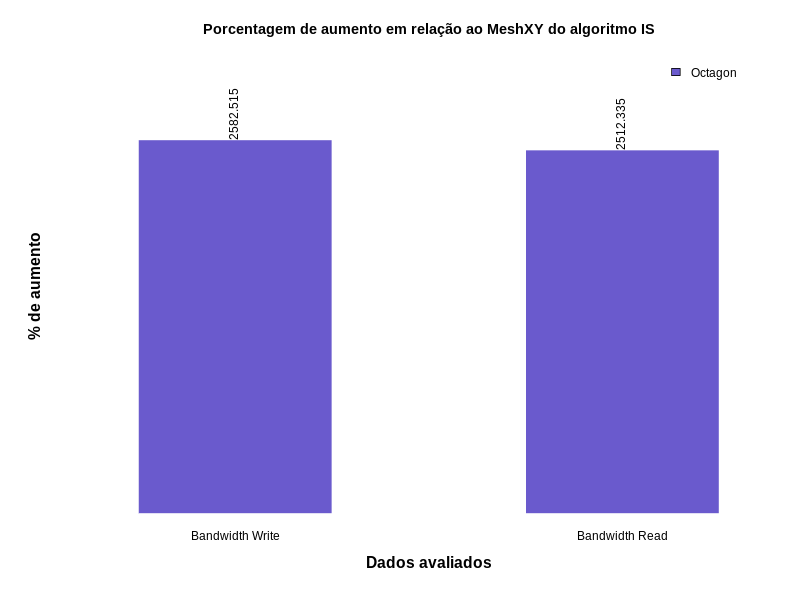
\includegraphics[width=15cm, height=9cm]{imagens/is2.png}
\label{foto2}
\caption{Porcentagem de aumento de vazão de leitura e escrita}
\end{figure}

\begin{figure}[H]
\centering
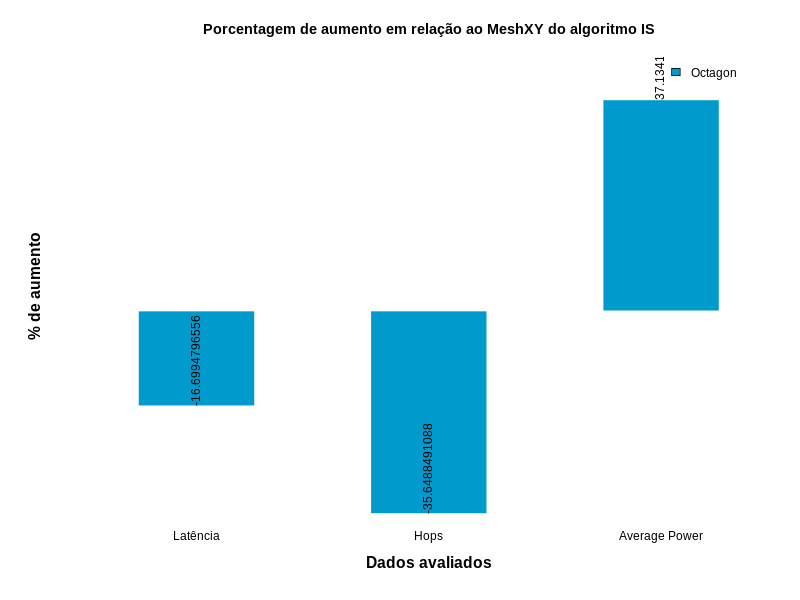
\includegraphics[width=15cm, height=9cm]{imagens/is.png}
\label{foto1}
\caption{Porcentagem de aumento de latência, saltos e força média}
\end{figure}

\section{Conclusão}\label{sec:conc}
 %Intro -> Solucao -> Objetivo  -> Metologia -> Resultados -> Concluiu
 As topologias de rede são usadas para mapear os caminhos que os dados devem seguir de forma mais eficiente, assim, o objetivo deste trabalho foi comparar duas topologias (Mesh e Octagon) e verificar seus desempenhos. 
 
 Para atingir este objetivo, utilizamos o simulador gem5 no modo \textit{system emulation}, rodando com cada topologia, os algoritmos IS, KM, Fast, FN, GF, LU e o TSP, retirados do CAPBenchmark.
 
 Ao fim, pôde-se observar que por conta da maior vazão, (ou seja, mais dados sendo processados de uma vez) da topologia octagon, obteve-se um ganho de aproximadamente 16\% na latência, e de aproximadamente 35\% no número de saltos tomados. Logo, a topologia octagon se mostrou mais eficiente. No entanto, por conta do número elevado de operações, tivemos um aumento de cerca de 37\% no consumo de energia.

\bibliographystyle{sbc}
\bibliography{main.bib}
\end{document}
